% %%%%%%%%%%%%%%%%%%%%%%%%%%%%%%%%%%%%%%%%%%%%%%%%%%%%%%%%%%%%%%%%%%%%%%%%%%%%%
% %%%%%%%%%%%%%%%%%%%%%%%%%%%%%%%%%%%%%%%%%%%%%% Description of Numerical Model
% %%%%%%%%%%%%%%%%%%%%%%%%%%%%%%%%%%%%%%%%%%%%%%%%%%%%%%%%%%%%%%%%%%%%%%%%%%%%%

\chapter{Numerical Model}
  \label{ch_model}

\todo{Sketch out this chapter. What does 2.5 dimensions mean? Why is it an appropriate approach to this problem? Why is this model in particular a good fit? What previous similar work has been done? What's novel about this mode? }

\todo{Also 2.5D: Waters 2013\cite{waters_2013}. And Waters 2008\cite{waters_2008}. }

Waters\cite{waters_2013} cites Olson\cite{olson_1978} with reference to modenumber. 

The model works in two and a half dimensions. A meridional slice of the magnetosphere is resolved. Fields are presumed to vary azimuthally according to a fixed modenumber \azm. Derivatives in $\phi$ are replaced by $i \azm$. Imaginary field values indicate a phase shift in the azimuthal direction. 

\todo{From Bob's 2013 paper\cite{lysak_2013} (which was also 2.5D): ``The shear \Alfven and compressional fast mode waves can be coupled not only by the Hall conductivity but also by inhomogeneities in the background plasma, which are unavoidable in a realistic magnetosphere [e.g., Lysak and Yoshikawa, 2006\cite{lysak_2006}; Waters et al., 2012\cite{waters_2013}]. This coupling requires a finite wave vector component in the azimuthal direction, i.e., a finite $m$ in the context of the present model. Because of the $\exp \arg{ i m \phi}$ dependence assumed in this model, the coupling from the inhomogeneity enters as an imaginary part of the coupled wave fields with respect to the initial fields, whereas the Hall conductivity appears in phase with the initial fields. Thus, although a fully three-dimensional model can give a more complete picture of wave propagation [e.g., Lysak, 2004\cite{lysak_2004}; Woodroffe and Lysak, 2012\cite{woodroffe_2012}], the present two-dimensional model serves to illustrate the nature of this coupling.''}

The use of a fixed modenumber allows a dramatic decrease in computational cost. Waves with very high azimuthal modenumber are prohibitively expensive to simulate since they can only be resolved if grid resolution is very fine in the azimuthal direction. 

\todo{Can we find a citation where someone explicitly talks about the computational cost of high-\azm simulations? Or is it just obvious Nyquist? }

This prevents the simultaneous consideration of dayside and nightside phenomena, but is fine for azimuthally-localized waves. As was shown by \cite{engebretson_1987}, and recently confirmed in detail by \cite{dai_2015}, Pc4 pulsations are generally confined to just a few hours MLT on the dayside. 

Driving with a compressional pulse from the outer boundary of a simulation is typical. This model also includes a novel driving mechanism: perturbations to the ring current. 

The code is linear. All magnetic fields are a first-order perturbation over the zeroth-order dipole field. This is a not-great assumption out towards the magnetopause. In practice, however, most activity is within $L \sim \SI{7}{\RE}$, where the dipole approximation is pretty good. 

Models with height-resolved ionospheres are a very recent development. Lysak presented his in 2013\cite{lysak_2013}. 

Ground signatures are fairly recent as well. 

\todo{Some ground signature work as far back as Greifinger and Greifinger in 1968\cite{greifinger_1968}, but there's been steady advancement. Lysak and Song, in 2006, were the first to work out ground signatures without the assumption of a single-frequency wave. }

\todo{The support software -- the driver and the plotter -- are significant too. Do they go in a section? In an appendix? }

\todo{Past FLR simulations focused on a single mode, didn't account well for the ionosphere, etc. Lee and Lysak 1989, 1990, 1991, Rankin et al 1993, 1995, 1999, Tikhonchuk and Rankin 2000, 2002. }

\todo{Past work that got ground signatures (without latitude-dependent zenith angle) Greifinger and Greifinger 1968, 1973, Hughes 1974, Sciffer and Waters 2002, Sciffer et al 2005. Better computation of ground signatures... Waters and Sciffer 2008, Sciffer and Waters 2011, Woodroffe and Lysak 2012. }

Note that the model uses megameters, seconds, megacoulombs, and grams as the fundamental units of length, time, charge, and mass respectively. As a result, electric field is measured in \si{\mV/\meter}, magnetic field is measured in \si{\nano\tesla}, and Poynting flux is measured in \si{\mW/\meter\squared}. The electric constant is expressed in \si{\milli\farad/\meter}, not in units of \ez, not that it really matters. 

% =============================================================================
% =============================================================================
% =============================================================================
\section{Coordinate System}
  \label{sec_coords}

\todo{Past work which could be cited for geometry examples: Radoski 1967, Lee and Lysak 1989, 1991, Rankin et al 1993, 1994, Streltsov and Lotko 1995, 1999. }

FLRs have traditionally been modeled by straightening the field lines into a rectangular configuration\cite{dungey_1954,mann_1995}, by unrolling the azimuthal coordinate into a cylindrical coordinate system\cite{radoski_1974}, or through the use of dipole coordinates\cite{radoski_1967_coords}\footnote{The dipole coordinates \radx, \rady\ and \radz are perhaps more commonly named $\mu$, $\phi$, and $\nu$ respectively; however, in the present work, $\mu$ and $\nu$ take other meanings.}:
\begin{align}
  \label{radoski_coords}
  \radx &\equiv -\frac{\sin^2 \theta}{r} &
  \rady &\equiv \phi &
  \radz &\equiv \frac{\cos \theta}{r^2}
\end{align}

Where $r$, $\theta$, and $\phi$ take on their usual spherical meanings of radial distance, colatitude, and azimuthal angle respectively. 

The dipole coordinate \radx is constant over each equipotential shell\footnote{In fact, \radx is inversely proportional to the McIlwain parameter.}, \rady is azimuthal angle, and \radz indexes each field line from south to north. The unit vectors \xhat, \yhat, and \zhat point in the crosswise\footnote{In the context of in situ measurements taken near the equatorial plane, \xhat is referred to as the radial direction; however, the present work extends the dipole grid to low altitudes, where it can be more horizontal than vertical. The term ``crosswise'' is meant to indicate that \xhat is defined by the cross product of \yhat and \zhat.} (radially outward at the equator), azimuthal (eastward), and parallel (northward at the equator) directions respectively. 

% -----------------------------------------------------------------------------
% -----------------------------------------------------------------------------
% -----------------------------------------------------------------------------
\subsection{Differential Geometry}
  \label{sec_geometry}

Notably, the dipole coordinates \radx, \rady, and \radz are normal to one another. While mathematically convenient, they do not readily accommodate a fixed-altitude boundary at the ionosphere, nor do they allow the dipole magnetic field to intersect the boundary at an oblique angle, as Earth's field does. As a solution, a nonorthogonal set of dipole coordinates was developed numerically by Proehl\cite{proehl_2002}, then formalized analytically by Lysak\cite{lysak_2004} in terms of their contravariant components:
\begin{align}
  \label{def_coords}
  \lysakx & = - \frac{R_I}{r} \sin^2 \theta & 
  \lysaky & = \phi &
  \lysakz & = \frac{R_I^2}{r^2} \frac{\cos \theta}{\cos \theta_0}
\end{align}

Above, $R_I$ is the position of the ionosphere relative to Earth's center; it's typically taken to be \SI{1}{\RE} + \SI{100}{\km}. 

Like the dipole coordinates \radx, \rady, and \radz, Lysak's coordinates \lysakx, \lysaky, and \lysakz correspond to $L$-shell, azimuthal angle, and position along a field line respectively. However, compared to \radz, \lysakz has been renormalized using the invariant colatitude\footnote{The invariant colatitude is the colatitude $\theta$ at which a field line intersects the ionosphere. It is related to the McIlwain parameter by $\cos\theta_0 \equiv \sqrt{1 - \frac{R_I}{L}}$. } $\theta_0$. As a result, \lysakz takes the value \num[retain-explicit-plus]{+1} at the northern ionospheric boundary and \num{-1} at the southern ionospheric boundary for all \lysakx and \lysaky. 

Because Lysak's coordinate system is not orthogonal\footnote{Curves of constant \lysakx and curves of constant \lysakz can intersect at non-right angles. }, it's necessary to consider covariant and contravariant basis vectors separately. 
\begin{align}
  \hat{e}_i & \equiv \dd{\lysaki} \vec{r} &
  \hat{e}^i & \equiv \dd{ \vec{r} } \lysaki
\end{align}

Covariant basis vectors $\hat{e}_i$ are normal to the curve defined by constant $\lysaki$, while contravariant basis vectors $\hat{e}^i$ are tangent to the coordinate curve (or, equivalently, $\hat{e}^i$ is normal to the plane defined by constant $u^j$ for all $j \ne i$). These vectors are reciprocal\footnote{The symbol $\delta^i_j$ is the Kronecker delta; the present work also makes use of the Levi-Civita symbol $\varepsilon^{ijk}$ and Einstein's convention of implied summation over repeated indeces\cite{einstein_1916}. } to one another, and can be combined to give components of the metric tensor $\tensor{g}$\cite{dhaeseleer_1991}. 
\begin{align}
  \label{def_metric}
  \hat{e}^i \cdot \hat{e}_j &= \delta^i_j &
  g_{ij} &\equiv \hat{e}_i \cdot \hat{e}_j &
  g^{ij} &\equiv \hat{e}^i \cdot \hat{e}^j 
\end{align}

The metric tensor allows rotation between covariant and contravariant representations of vectors. 
\begin{align}
  \label{metric}
  A_i &= g_{ij} A^j &
  & \text{and} &
  A^i &= g^{ij} A_j &
  & \text{where} &
  A_i &\equiv \vec{A} \cdot \hat{e}_i &
  & \text{and} &
  A^i &\equiv \vec{A} \cdot \hat{e}^i
\end{align}

In addition, the determinant of the metric tensor\footnote{Note $g \equiv \det \tensor{g}$. } is used to define cross products and curls\footnote{The quantity \jac is called the Jacobian determinant. It's sometimes denoted using the letter $J$, which the present work reserves for current.}. 
\begin{align}
  \label{jacobian}
  \lr{ \cross{A}{B} }^i &= \frac{ \varepsilon^{ijk} }{\jac} A_j B_k &
  & \text{and} &
  \lr{ \curl{A} }^i &= \frac{ \varepsilon^{ijk} }{\jac} \dd{\lysakj} A_k &
  & \text{where} &
  \jac &= \sqrt{g}
\end{align}

Explicit forms of the basis vectors and metric tensor can be found in the appendix of \cite{lysak_2004}. At present, it's sufficient to note the mapping between Lysak's basis vectors and the usual dipole unit vectors. 
\begin{align}
  \label{def_xyz_directions}
  \xhat &= \frac{1}{ \sqrt{ g^{11} } } \hat{e}^1 &
  \yhat &= \frac{1}{ \sqrt{ g^{22} } } \hat{e}^2 &
  \zhat &= \frac{1}{ \sqrt{ g_{33} } } \hat{e}_3
\end{align}

The basis vectors can also be mapped to the spherical unit vectors, though \cref{def_rqf_directions} is valid only at the ionospheric boundary. 
\begin{align}
  \label{def_rqf_directions}
  \qhat &= \frac{1}{ \sqrt{ g_{11} } } \hat{e}_1 &
  \fhat &= \frac{1}{ \sqrt{ g_{22} } } \hat{e}_2 &
  \rhat &= \frac{1}{ \sqrt{ g^{33} } } \hat{e}^3
\end{align}

% -----------------------------------------------------------------------------
% -----------------------------------------------------------------------------
% -----------------------------------------------------------------------------
\subsection{Numerical Application}
  \label{sec_grid}

The coordinates converge at the equatorial ionosphere, so an inner boundary is necessary to maintain finite grid spacing. It's typically placed at $L=2$. The outer boundary is at $L=10$. The dipole approximation of Earth's magnetic field is tenuous at the outer boundary (particularly on the dayside); however, in practice, wave activity is localized inside $L\sim7$. The grid is spaced uniformly in \lysakx, which gives finer resolution close to Earth and coarser resolution at large distances. 

Spacing in \lysakz is set by placing grid points along the outermost field line. The points are closest together at the ionosphere, and grow towards the equator. The spacing increases in a geometric fashion, typically by \SI{3}{\percent}. 

Most simulations take the grid to be 150 points in \lysakx by 350 points in \lysakz. The result is a resolution on the order of \SI{10}{\km} at the ionosphere, which increases to the order of \SI{e3}{\km} at the midpoint of the outermost field line. 

There are no grid points in \lysaky, of course, because of the two and a half dimensional nature of the model. Fields are assumed to vary as $\exp \arg{i \azm \lysaky}$, so derivatives with respect to \lysaky are equivalent to a factor of $i \azm$. In effect, this means that the real component of each field is azimuthally in phase with the (purely real) driving, while imaginary values represent behavior that is azimuthally offset. 

\begin{figure}[H]
    \centering
    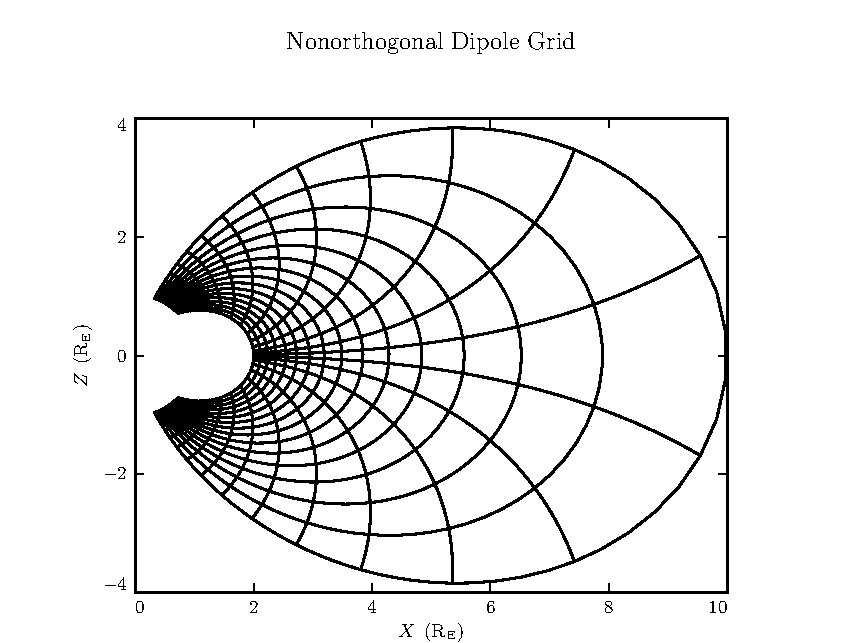
\includegraphics[width=\textwidth]{figures/grid.pdf}
    \caption[Nonorthogonal Dipole Grid]{
      The model's nonorthorthogonal dipole grid. Every fifth point is shown in each direction. The high concentration of grid points near Earth's equator is a consequence of the coordinate system, which converges at the equatorial ionosphere. 
    }
    \label{fig_grid}
\end{figure}

The simulation's time step is set based on the grid spacing. As is the convention, \dt is set to match the smallest \Alfven zone crossing time, scaled down by a Courant factor (typically 0.1). It bears noting that the smallest crossing time need not correspond to the smallest zone; recall from \cref{fig_va} that the \Alfven speed is very high in the Ionospheric \Alfven Resonator. A typical time step is on the order of \SI{e-5}{\second}. 

\todo{Do we need a citation for how time steps are set based on crossing times? }

% =============================================================================
% =============================================================================
% =============================================================================
\section{Maxwell's Equations}
  \label{sec_eqns}

\todo{Introduce \farlaw and \amplaw, respectively, after using Kirchhoff's formulation of \ohmlaw ($\vec{J} = \tensor{\sigma} \cdot \vec{E}$) to eliminate explicit curl dependence... which will be revisited in \cref{ch_inertia}. }
\begin{align}
  \label{def_eqns}
  \ddt \vec{B} &= - \curl{E} &
  \tensor{\epsilon} \cdot \ddt \vec{E} &= \frac{1}{\mu_0} \curl{B} - \tensor{\sigma} \cdot \vec{E}
\end{align}

\todo{Explain that we'll start in \x-\y-\z coordinates -- crosswise, azimuthal, and parallel -- then map to the nonorthogonal basis at the very end. Otherwise it's necessary to carry around geometric factors. }

% -----------------------------------------------------------------------------
% -----------------------------------------------------------------------------
% -----------------------------------------------------------------------------
\subsection{Linearization and Optimization}
  \label{sec_optimization}

\todo{Leapfrog grid (for which Waters\cite{waters_2013} cites Taflove and Hagness, an electrodynamics textbook). Talk about the grid parity as well as the offset in time. }

%Field values are offset to ensure that most differences are centered. For example, $\ddt B_2$ depends on $\dd{\lysakx} E_3$ and $\dd{\lysakz} E_1$. If $B_2$ is defined at even $i$, $E_3$ is defined at odd $i$, so that $B_2$ is defined on the same grid points as $\frac{ E_3 \lrb{i+1} - E_3 \lrb{i-1} }{ \lysakx \lrb{i+1} - \lysakx \lrb{i-1} }$. 

%\todo{Make sure the example uses the currect parities. }

%\todo{Find a citation for the wigglies that occur if field values are defined on all grid points, due to the weak coupling. This problem is apparently well-known. }

%Values are sometimes needed off-parity. $E_1$ and $E_2$ are not defined at the same grid locations, but they are coupled directly by the Hall conductivity. And $B_1$ and $B_3$ are coupled by the non-orthogonality of the grid. When off-parity values are needed, they are interpolated from their neighbors. 

%Differentiation and interpolation are good to second order on the nonuniform grid. Like the coefficients for Maxwell's equations, differentiation and interpolation weights are computed during setup to save time during iteration. 

%\begin{align}
%  \label{def_assign}
%  \begin{split}
%  \int_0^{\dt} \! dt \, \ddt \vec{B} &= - \displaystyle\int_0^{\dt} \! dt \, \curl{E} \\ 
%  \left. \vec{B} \right|_{\dt} - \left. \vec{B} \right|_0 &= \left. - \dt \, \curl{E} \right|_{ \frac{\dt}{2} } \\
%  \vec{B} &\assign \vec{B} - \dt \, \curl{E}
%  \end{split}
%\end{align}

\todo{Precomputation of coefficients. }

\todo{Curl shorthand, \vec{C} and \vec{F}. Recalling \cref{jacobian}, }
\begin{align}
  \label{def_curls}
  C^i & = \frac{ \varepsilon^{ijk} }{\jac} \dd{\lysakj} E_k &
  F^i & = \frac{ \varepsilon^{ijk} }{\jac} \dd{\lysakj} B_k
\end{align}

\todo{OpenMP. }

\todo{Keeping only covariant field components and contravariant curl components, since we only use contravariant coordinates. }

% -----------------------------------------------------------------------------
% -----------------------------------------------------------------------------
% -----------------------------------------------------------------------------
\subsection{Magnetic Fields}
  \label{sec_b}

Taking the shorthand introduced in \cref{def_curls}, \farlaw can simply be written: 
\begin{align}
  \label{farlaw_ijk}
  \ddt B^i &= - C^i
\end{align}

Writing each component out explicitly, and using the metric tensor (per \cref{metric}) to eliminate contravariant magnetic field components, \cref{farlaw_ijk} becomes:
\begin{align}
  \label{farlaw_final}
  \begin{split}
  B_1 &\assign B_1 - g_{11} \, \dt \, C^1 - g_{13} \, \dt \, C^3 \\
  B_2 &\assign B_2 - g_{22} \, \dt \, C^2 \\
  B_3 &\assign B_3 - g_{31} \, \dt \, C^1 - g_{33} \, \dt \, C^3
  \end{split}
\end{align}

Note that the \assign operator is used in \cref{farlaw_final} to indicate assignment, rather than equality. Terms on the left are new, while those on the right are old. 

% -----------------------------------------------------------------------------
% -----------------------------------------------------------------------------
% -----------------------------------------------------------------------------
\subsection{Electric Fields}
  \label{sec_e}

\amplaw, as formulated in \cref{def_eqns}, presents a nontrivial differential equation. Not only are the electric field values coupled to their own derivatives, but the crosswise and azimuthal components of the equation are coupled by the Hall terms in the conductivity tensor. 

Fortunately, the permittivity tensor can be easily inverted, allowing a solution by integrating factor. Recalling the shorthand introduced in \cref{def_curls},
\begin{align}
  \label{int_fac_0}
  \tensor{\epsilon} \cdot \ddt \vec{E} &= \frac{1}{\mu_0} \vec{F} - \tensor{\sigma} \cdot \vec{E} &
  & \text{becomes} &
  \lr{ \tensor{\Omega} + \tensor{ \mathbb{I} } \ddt } \cdot \vec{E} &= \vec{V}^2 \cdot \vec{F}
\end{align}

Where $\tensor{ \mathbb{I} }$ is the identity tensor and in \x-\y-\z coordinates, 
\begin{align}
  \tensor{V}^2 &\equiv \frac{1}{\mz} \tensor{\epsilon}^{-1} = 
    \mmm{\va^2}{0}{0}
        {0}{\va^2}{0}
        {0}{0}{c^2}
  && \text{and} &
  \tensor{\Omega} &\equiv \tensor{\epsilon}^{-1} \cdot \tensor{\sigma} = 
    \mmm{ \frac{\sp}{\ep} }{ \frac{-\sh}{\ep} }{0}
        { \frac{\sh}{\ep} }{ \frac{\sp}{\ep} }{0}
        {0}{0}{ \frac{\sz}{\ez} } 
\end{align}

Multiplying through by $\exp \arg{ \tensor{\Omega} \, t }$ and applying the product rule, \cref{int_fac_0} becomes\footnote{Tensor exponentiation is analogous to scalar exponentiation\cite{hall_2015}: $\exp \arg{ \tensor{T} } \equiv \displaystyle\sum_n \frac{1}{ n! } \tensor{T}^n$.}
\begin{align}
  \label{int_fac_1}
  \ddt \Big( \exp \arg{\tensor{\Omega} \, t} \cdot \vec{E} \, \Big) &= \exp \arg{\tensor{\Omega} \, t} \cdot \vec{V}^2 \cdot \vec{F}
\end{align}

\cref{int_fac_1} can then be integrated over a small time step \dt and expressed in terms of the assignment operator introduced in \cref{farlaw_ijk}. 
\begin{align}
  \label{int_fac_2}
  \vec{E} &\assign \exp \arg{ -\tensor{\Omega} \, \dt } \cdot \vec{E} + \dt \, \exp \arg{ -\tensor{\Omega} \, \tfrac{\dt}{2} } \cdot \tensor{V}^2 \cdot \vec{F}
\end{align}

The tensor exponential can be evaluated by splitting $\tensor{\Omega}$ into the sum of its diagonal and Hall components\footnote{As long as the tensors $\tensor{T}$ and $\tensor{T}'$ commute -- which is guaranteed if either is diagonal -- $\exp \arg{ \tensor{T} + \tensor{T}' } = \exp \arg{ \tensor{T} } \exp \arg{ \tensor{T}' }$. }. The Hall exponential condenses into sines and cosines, giving a rotation around the magnetic field line. 
\begin{align}
  \label{amp_final}
  \vec{E} &\assign \exp \arg{ -\tensor{\Omega}_D \; \dt } \cdot \tensor{R}_z \arg{ \tfrac{-\sh \dt}{\ep} } \cdot \vec{E}
   + \dt \, \tensor{V}^2 \cdot \exp \arg{ -\tensor{\Omega}_D \; \tfrac{\dt}{2} } \cdot \tensor{R}_z \arg{ \tfrac{-\sh \dt}{2 \ep} } \cdot \vec{F}
\end{align}

Where 
\begin{align}
  \tensor{R}_z \arg{\theta} &= 
  \mmm{\cos\theta}{-\sin\theta}{0}
      {\sin\theta}{\cos\theta}{0}
      {0}{0}{1} &
  & \text{and} &
  \tensor{\Omega}_D &\equiv
    \mmm{ \frac{\sp}{\ep} }{0}{0}
        {0}{ \frac{\sp}{\ep} }{0}
        {0}{0}{ \frac{\sz}{\ez} }
\end{align}

The parallel component of term of \cref{amp_final} is simply
\begin{align}
  E_\parallel \assign E_\parallel \exp \arg{ \tfrac{- \sz \dt}{\ez} } + c^2 \dt F_\parallel \exp \arg{ \tfrac{- \sz \dt}{2 \ez} }
\end{align}

Or, in covariant terms, 
\begin{align}
  \label{e3_final}
  E_3 \assign E_3 \exp \arg{ \tfrac{- \sz \dt}{\ez} } + c^2 \dt \lr{ g_{31} F^1 + g_{33} F^3 } \exp \arg{ \tfrac{- \sz \dt}{2 \ez} }
\end{align}

Using the conductivity profiles introduced in \cref{sec_ionos}, the minimum value of $\frac{\sz \dt}{\ez}$ is on the order of \num{e3}, making $\exp \arg{ \frac{- \sz \dt}{\ez} }$ far too small to be stored in a double precision variable\footnote{Not coincidentally, $\frac{\sz}{\ez}$ can also be written $\frac{\op^2}{\nu}$. At the ionosphere, the collision frequency $\nu$ is fast compared to the frequency of a ULF wave... but it's still slow compared to the plasma frequency.}. That is, this model takes $E_3$ (and, proportionally, $E_\parallel$) to be uniformly zero. This issue is revisited in \cref{ch_inertia}. 

The perpendicular components of \cref{amp_final}, mapped from the dipole basis to the covariant basis using \cref{def_xyz_directions} and \cref{metric}, give the expressions: 
\begin{alignat}{6}
  \label{e1_final}
  & E_1 + \frac{ g^{13} }{ g^{11} } && E_3 \assign &&   && E_1 && \cos \arg{ \tfrac{- \sh \dt}{\ep} } \exp \arg{ \tfrac{- \sp \dt}{\ep} } &&  \notag \\
  &                                 &&             && + && E_2 && \sin \arg{ \tfrac{- \sh \dt}{\ep} } \exp \arg{ \tfrac{- \sp \dt}{\ep} } &&  \sqrt{ \frac{ g^{22} }{ g^{11} } } \notag \\
  &                                 &&             && + && E_3 && \cos \arg{ \tfrac{- \sh \dt}{\ep} } \exp \arg{ \tfrac{- \sp \dt}{\ep} } &&  \frac{ g^{13} }{ g^{11} } \\
  &                                 &&             && + && F^1 && \cos \arg{ \tfrac{- \sh \dt}{2\ep} } \exp \arg{ \tfrac{- \sp \dt}{2\ep} } &&  \frac{\va^2 \dt}{ g^{11} } \notag \\
  &                                 &&             && + && F^2 && \sin \arg{ \tfrac{- \sh \dt}{2\ep} } \exp \arg{ \tfrac{- \sp \dt}{2\ep} } &&  \frac{\va^2 \dt}{ \sqrt{ g^{11} g^{22} } } \notag \\
  \intertext{and}
  \label{e2_final}
  & && E_2 \assign && - && E_1 && \sin \arg{ \tfrac{- \sh \dt}{\ep} } \exp \arg{ \tfrac{- \sp \dt}{\ep} } &&  \sqrt{ \frac{ g^{11} }{ g^{22} } } \notag \\
  & &&             && + && E_2 && \cos \arg{ \tfrac{- \sh \dt}{\ep} } \exp \arg{ \tfrac{- \sp \dt}{\ep} } &&  \notag \\
  & &&             && - && E_3 && \sin \arg{ \tfrac{- \sh \dt}{\ep} } \exp \arg{ \tfrac{- \sp \dt}{\ep} } &&  \frac{ g^{13} }{ \sqrt{ g^{11} g^{22} } } \\
  & &&             && - && F^1 && \sin \arg{ \tfrac{- \sh \dt}{2\ep} } \exp \arg{ \tfrac{- \sp \dt}{2\ep} } &&  \frac{\va^2 \dt}{ \sqrt{ g^{11} g^{22} } } \notag \\
  & &&             && + && F^2 && \cos \arg{ \tfrac{- \sh \dt}{2\ep} } \exp \arg{ \tfrac{- \sp \dt}{2\ep} } &&  \frac{\va^2 \dt}{ g^{22} } \notag
\end{alignat}

Note that the $E_3$ terms can be ignored at present. They are referenced in \cref{ch_inertia}. 

% =============================================================================
% =============================================================================
% =============================================================================
\section{Driving}
  \label{sec_driving}

\todo{If no energy is added, the simulation is pretty boring. Everything just stays zero. }

% -----------------------------------------------------------------------------
% -----------------------------------------------------------------------------
% -----------------------------------------------------------------------------
\subsection{Outer Boundary Compression}

\todo{It's traditional to drive from the outer boundary. Cite some examples. It's an analog for solar wind conditions. The analogy is clear at low modenumbers (large azimuthal wavelengths), but is plausible at high modenumber (small azimuthal wavelengths) as well, due to KH waves on the magnetopause, for example. }

\todo{As discussed in \cref{ch_pc4s} and again in \cref{sec_math_implications}, \Alfven waves become guided as the azimuthal modenumber becomes large. Energy delivered at the outer boundary, as a result, is unable to propagate across field lines to stimulate resonances in the inner magnetosphere.}

\todo{Compressional driving is applied by setting the value of $B_3$ at the boundary. A typical scale is \SI{10}{\nano\tesla}. }

\todo{\cref{fig_bdrive} demonstrates this issue. Note that the large values on the bottom row should be taken with a grain of salt; it's not clear that the simulation is reliable when waves are continuously forced against the boundary. }

\begin{figure}[H]
    \centering
    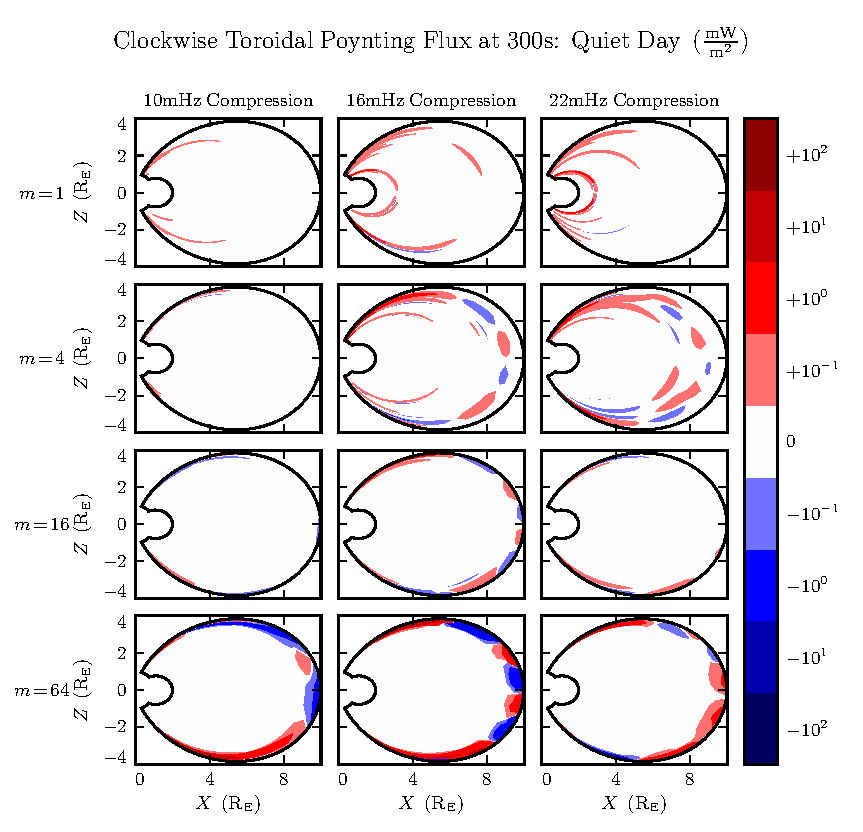
\includegraphics[width=\textwidth]{figures/Stor_B_2.pdf}
    \caption[Decreasing Penetration with Increasing Modenumber]{
      When the azimuthal modneumber is small, energy delivered through compression at the outer boundary propagates across field lines to stimulate resonances in the inner magnetosphere. However, as modenumber increases, \Alfven waves become increasingly guided. As a result, the inner magnetosphere is unaffected by perturbations at the outer boundary. 
    }
    \label{fig_bdrive}
\end{figure}

\todo{The present work, as a result, focuses mostly on simulations driven from within the magnetosphere. }

% -----------------------------------------------------------------------------
% -----------------------------------------------------------------------------
% -----------------------------------------------------------------------------
\subsection{Ring Current Modulation}

\todo{Pc4 pulsations with high azimuthal modenumber have been shown to originate within the magnetosphere, such as through drift-resonant interactions with energetic radiation belt and ring current particles. Substorm injection can cause localized ring current behavior. }

\todo{During and after geomagnetically active times, the ring current is a dynamic region. It's easy to imagine localized perturbations, though difficult to estimate their scale. The following is a kludgey estimate -- better than no estimate at all! }

\todo{The Sym-H storm index\cite{nasa_cdaweb} measures magnetic perturbations on Earth's surface due to ring current activity. It's measured once per minute\footnote{Dst, the more commonly used storm index, is measured hourly. }, so Fourier amplitudes in the Pc4 range cannot be measured directly. However, they can be inferred by fitting the pink noise distribution. \cref{fig_symh} shows a Fourier series of the June 2013 storm and its recovery, along with its Fourier series coefficients. The red line shows a fit along the maximum of the Fourier coefficients. }

\todo{Note that Sym-H is global and we're looking at localized perturbations! This is a conservative estimate, because it's averaged over the entire globe. Information on modenumbers comes from observations by Dai\cite{dai_2015} and Takahashi\cite{takahashi_2013}, both of whom have seen fundamental-mode Pc4 pulsations with modenumbers of $\sim\num{70}$. }

\begin{figure}[H]
    \centering
    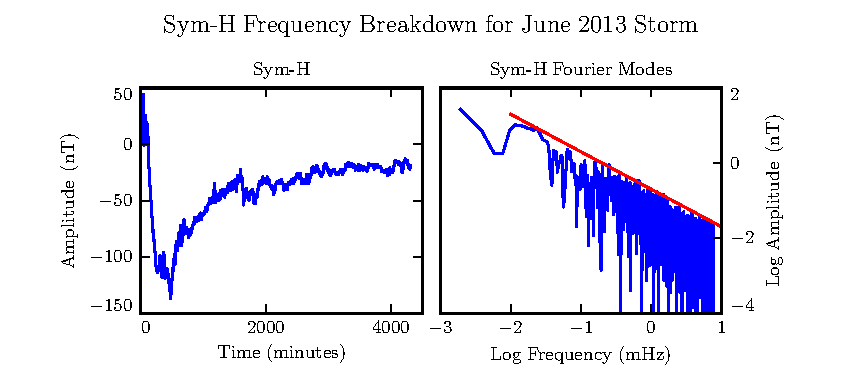
\includegraphics[width=\textwidth]{figures/symh.pdf}
    \caption[Sym-H Fourier Components for June 2013 Storm ]{
      The Sym-H storm index\cite{nasa_cdaweb} measures magnetic perturbations on Earth's surface due to ring current activity. The amplitude of oscillations in the Pc4 range is estimated by fitting the Fourier amplitudes of the June 2013 storm. 
    }
    \label{fig_symh}
\end{figure}

\todo{$\tilde{B} \arg{f} \sim \SI{e-2}{\nano\tesla} \lr{ \frac{ \SI{20}{\mHz} }{f} }$. }

\todo{An oscillation with a period of about a minute could have an amplitude on the order of \SI{e-2}{\nano\tesla}. }

\todo{Driving is typically delivered at $L=5$, with a Gaussian spread of \SI{0.5}{\RE} radially and \SI{5}{\degree} in latitude. Estimating the geometric factors from the size of the ring current, and from the fact that Sym-H is measured at Earth's surface rather than at the center of the ring, this gives current density on the order of \SI{e-4}{\uA/\meter\squared}. }

\todo{The driving current is applied by splitting the current in \amplaw into an Ohmic term and a driving term: 
\begin{align}
  \tensor{\epsilon} \cdot \ddt \vec{E} &= \frac{1}{\mu_0} \curl{B} - \tensor{\sigma} \cdot \vec{E} - \vec{J}_{drive}
\end{align}
\cref{def_curls} is then ammended so that $\vec{F} \equiv \curl{B} - \vec{J}_{drive}$. As a result, no changes are necessary to \cref{e1_final,e2_final,e3_final}. 
}

\todo{Effective peak driving electric field is... }

% =============================================================================
% =============================================================================
% =============================================================================
\section{Boundary Conditions}
  \label{sec_bcs}

\todo{The grid can't go on forever. There have to be special cases at the edges. }

% -----------------------------------------------------------------------------
% -----------------------------------------------------------------------------
% -----------------------------------------------------------------------------
\subsection{Inner and Outer Bounadries}

\todo{Recall that parity was already discussed in \cref{sec_optimization}. }

Dirichlet and Neumann boundary conditions are applied to the electric field components and magnetic field components respectively. That is, electric fields are forced to go to zero at the inner and outer boundaries, and magnetic fields are forced to have a zero derivative normal to the inner and outer boundaries. 

These boundary conditions can in principle cause nonphysical reflections at the boundary\footnote{See, for example, the bottom row of \cref{fig_bdrive}. }. However, in practice, wave activity is concentrated well within the simulation domain. Simulation results are robust under an exchange of Dirichlet and Neumann boundary conditions (though a self-inconsistent set of boundary condidtions, such as applying Neumann boundary conditions to $B_1$ but Dirichlet boundary conditions to $B_3$, quickly causes instability). 

% -----------------------------------------------------------------------------
% -----------------------------------------------------------------------------
% -----------------------------------------------------------------------------
\subsection{Coupling to the Atmosphere}

Between the top of the neutral atmosphere and the bottom of the ionosphere, the model includes a thin, horizontal current sheet representing the ionosphere's $E$ layer\cite{lysak_2004}. By integrating \amplaw over the layer, it can be shown\cite{fujita_1988} that the horizontal electric field values at the edge of the grid are determined by the jump in the horizontal magnetic fields:
\begin{align}
  \label{jump_condition}
  \tensor{\Sigma} \cdot \vec{E} &= \displaystyle\lim_{\dr \rightarrow 0} \, \left[ \, \frac{1}{\mz} \hat{r} \! \times \! \vec{B} \, \right|^{R_I + \dr}_{R_I - \dr}
\end{align}

Like the height-resolved conductivities in \cref{sec_e}, the tensor $\tensor{\Sigma}$ is based on Kelley's\cite{kelley_1989} conductivity profiles. Parallel, Pedersen, and Hall conductivities are integrated from Earth's surface to the ionospheric boundary, then arranged (in $\theta$-$\phi$ coordinates) as\cite{lysak_2004}:
\begin{align}
  \label{def_sigma}
  \tensor{\Sigma} &\equiv \mm{ \frac{\Sigma_0 \Sigma_P}{ \Sigma_0 \cos^2 \alpha + \Sigma_P \sin^2 \alpha } }{ \frac{-\Sigma_0 \Sigma_H}{ \Sigma_0 \cos^2 \alpha + \Sigma_P \sin^2 \alpha } }
                             { \frac{\Sigma_0 \Sigma_H}{ \Sigma_0 \cos^2 \alpha + \Sigma_P \sin^2 \alpha } }{ \Sigma_P + \frac{\Sigma_H^2 \sin^2 \alpha}{ \Sigma_0 \cos^2 \alpha + \Sigma_P \sin^2 \alpha } } \end{align}

Where $\alpha$ is the angle between the magnetic field and the vertical direction, given by $\cos \alpha \equiv \frac{ -2 \cos \theta }{ \sqrt{1 + 3 \cos^2\theta} }$. 

An expression for the horizontal electric fields at the boundary can be obtained by inverting \cref{jump_condition}. After mapping to covariant coordinates per \cref{def_rqf_directions}, and taking $\Sigma \equiv \det \tensor{\Sigma}$,
\begin{align}
  \label{eatm_final}
  \begin{alignedat}{6}
  & E_1 \assign \frac{1}{\mz \Sigma} \bigg[ &- & \Sigma_{\theta\phi} && B_1   && - \sqrt{ \frac{ g_{11} }{ g_{22} } }&&\Sigma_{\phi\phi} && B_2 \bigg|^{R_I + \dr}_{R_I - \dr} \\
  & E_2 \assign \frac{1}{\mz \Sigma} \bigg[ &\sqrt{ \frac{ g_{22} }{ g_{11} } } & \Sigma_{\theta\theta} && B_1 && +  &&\Sigma_{\phi\theta} && B_2 \bigg|^{R_I + \dr}_{R_I - \dr}
  \end{alignedat}
\end{align}

The atmospheric magnetic field is computed as a linear combination of harmonics. The neutral atmosphere is considered to be a perfect insulator, giving $\curl{B}=0$. Combined with $\div{B}=0$ (per Maxwell's equations), this allows the computation of a magnetic scalar potential $\Psi$ such that $\vec{B}=\grad{\Psi}$ and $\Psi$ satisfies Laplace's equation, $\nabla^2 \Psi = 0$. 

Laplace's equation can be solved analytically; however, a numerical solution is preferrable to ensure orthonormality on a discrete and incomplete\footnote{As discussed in \cref{sec_coords}, the grid is constrained to finite $L$, which excludes the equator as well as the poles. } grid. After separating out the radial and azimuthal dependence in the usual way, the latitudinal component of Laplace's equation can be written in terms of $s \equiv - \sin^2 \theta$: 
\begin{align}
  \label{laplace}
  \lr{ 4 s^2 + 4s } \frac{d^2}{ds^2} Y_\ell + \lr{ 4 + 6 s } \frac{d}{ds} Y_\ell - \frac{\azm^2}{s} Y_\ell &= \ell \lr{ \ell + 1 } Y_\ell
\end{align}

Using centered differences to linearize the derivatives, \cref{laplace} becomes a system of coupled linear equations, one per field line. It can be solved numerically for eigenvalues $\ell \lr{\ell + 1}$ and eigenvectors\footnote{The eigenvectors are not vectors in the same sense as \vec{B} and \vec{E}, of course; rather, they are scalar functions of $\theta$ defined on a discrete grid.} $Y_\ell$\footnote{Solving Laplace's equation analytically results in spherical harmonics indexed by both $\ell$ and \azm, the separation constants for $\theta$ and $\phi$ respectively. In two and a half dimensions, $\phi$ is not explicitly resolved, so \azm is set manually.}. In terms of the harmonics $Y_\ell$, $\Psi$ between the Earth's surface and the top of the atmosphere can be written
\begin{align}
  \label{psi_expansion}
  \Psi \arg{r, \theta} &= \displaystyle\sum_\ell \lr{ a_\ell \, r^\ell + b_\ell \, r^{-\ell - 1} } Y_\ell \arg{\theta}
\end{align}

As a boundary condition for $\Psi$, Earth is assumed to be a perfect conductor. This forces the magnetic field at Earth's surface to be horizontal; that is, $B_r = \dd{r} \Psi = 0$. Noting that solutions to Laplace's equation are orthonormal, each element of the sum in \cref{psi_expansion} must be independently zero at $R_E$. This allows the coefficients $a_\ell$ and $b_\ell$ to be expressed in terms of one another. 
\begin{align}
  \label{beta_solution}
  b_\ell &= \frac{\ell}{\ell + 1} R_E^{2 \ell + 1} a_\ell
\end{align}

The current sheet at the top of the atmosphere has been assumed to be horizontal, so the radial component of the magnetic field must be the same just above and just below it. Taking the radial derivative of \cref{psi_expansion} at the top of the atmosphere, and eliminating $b_\ell$ with \cref{beta_solution}, gives
\begin{align}
  B_r &= \displaystyle\sum_\ell \ell \, \alpha_\ell \, R_I^{\ell-1} \, \lr{ 1 - \lambda_I^{2 \ell - 1} } Y_\ell &
  & \text{where} &
  \lambda_I &\equiv \frac{R_E}{R_I} \sim \num{0.975}
\end{align}

The summation can be collapsed by ``integrating'' over a harmonic. Inverse harmonics can be obtained by inverting the eigenvector matrix. Then $Y_\ell \cdot Y_{\ell'}^{-1} = \delta_{\ell \ell'}$ by construction. 
\begin{align}
  \label{alpha_solution}
  \alpha_\ell &= \frac{ 1 }{\ell \, R_I^{\ell-1} } \frac{ B_r \cdot Y_\ell^{-1} }{ 1 + \lambda_I^{2 \ell + 1} }
\end{align}

\todo{A dot product doesn't seem like great notation for the inner product of this sort of ``vector.'' What are better options? }

Combining \cref{psi_expansion,beta_solution,alpha_solution} allows the expression of $\Psi$ at the top and bottom of the atmosphere as a linear combination of radial magnetic field components at the bottom of the ionosphere. 
\begin{align}
  \label{psi_final}
  \begin{split}
  \Psi_E &= \displaystyle\sum_\ell Y_\ell \; \frac{R_I}{\ell} \frac{ \frac{2 \ell - 1}{\ell - 1} \lambda^\ell }{ 1 - \lambda_I^{2 \ell + 1} } B_r \cdot Y_\ell^{-1} \\
  \Psi_I &= \displaystyle\sum_\ell Y_\ell \; \frac{R_I}{\ell} \frac{ 1 + \frac{\ell}{\ell - 1} \lambda_I^{2 \ell + 1} }{ 1 - \lambda_I^{2 \ell + 1} } B_r \cdot Y_\ell^{-1}
  \end{split}
\end{align}

Horizontal magnetic fields are obtained by taking derivatives of $\Psi$. 
\begin{align}
  B_1 &= \dd{\lysakx} \Psi &
  B_2 &= \dd{\lysaky} \Psi
\end{align}

Horizontal magnetic field values at the top of the atmosphere are used to impose boundary conditions on the electric fields at the bottom of the ionosphere, per \cref{eatm_final}. Those at Earth's surface are valuable because they allow a direct comparison between model output and ground magnetometer data. 


